\documentclass[11pt]{article}

% ---------------------------------------------------------------------------
% Reward-Free Self-Prediction Drops Exogenous Control-Relevant Features:
% A Controlled Study
% Single-column, 11pt, clean article class (TMLR-style spirit; no proprietary
% .sty required). All numbers are traceable to PAPER_FACTS.md / result JSONs.
% ---------------------------------------------------------------------------

\usepackage[utf8]{inputenc}
\usepackage[T1]{fontenc}
\usepackage{microtype}
\usepackage[margin=1in]{geometry}
\usepackage{booktabs}
\usepackage{makecell}
\usepackage{graphicx}
\usepackage{amsmath}
\usepackage{amssymb}
\usepackage{siunitx}
\usepackage{xcolor}
\usepackage{hyperref}
\usepackage[round]{natbib}

\graphicspath{{figures/}}
\emergencystretch=1.5em  % absorb long unbreakable tokens (arXiv ids, \texttt names)

\hypersetup{
  colorlinks=true,
  linkcolor=blue!50!black,
  citecolor=blue!50!black,
  urlcolor=blue!50!black
}

\newcommand{\cellfour}{cell~4}
\newcommand{\probe}{linear-probe accuracy}

\title{\textbf{Reward-Free Self-Prediction Drops Exogenous\\ Control-Relevant Features: A Controlled Study}}

\author{
  Anonymous Author(s)\\
  \texttt{anon@example.org}
}

\date{}

\begin{document}
\maketitle

\begin{abstract}
\noindent
Joint-embedding predictive (JEPA-style) objectives learn representations by predicting future
latents, and in doing so they drop features that are \emph{exogenous}---uncontrollable by the
agent---yet control-relevant, even when those features are trivially encodable, because the
objective prices temporal predictability rather than control-relevance. We isolate this failure
in a controlled $2\times2$ experimental design that varies feature controllability and relevance
independently, equipped with a \emph{predictability knob} that decouples a feature's temporal
predictability from its control-relevance. Across six objectives---reconstruction, JEPA,
action-conditioned JEPA, controllability-based JEPA, inverse dynamics under a random policy, and
reward-grounded JEPA---every reward-free self-prediction objective fails to retain the
\emph{exogenous control-relevant feature} (\probe{} $\approx 0.51$, InfoNCE mutual information
$\approx 0$ nats), whereas reward-grounded prediction retains it selectively (probe $1.00$,
$\mathrm{MI}=0.693$ nats $=\log 2$, the maximum for a one-bit feature). The fix is label-efficient
and robust: as little as $2\%$ of transitions carrying a reward label suffices to recover the
feature, the effect holds across two environments with different surface forms, and it persists
across latent dimensions from $16$ to $1024$. At JEPA convergence the empirical bisimulation error
between analytically distinct feature classes is $1.893$ out of a maximum of $\approx 2.0$---a
near-maximal violation---indicating that the dropped information is exactly the reward-relevant
structure that bisimulation theory says an optimal representation should keep.
\end{abstract}

% ===========================================================================
\section{Introduction}
% ===========================================================================

A representation can fail a downstream task not because it lost something irrelevant, but because
it lost something it could not predict. Consider a feature that is simultaneously
\emph{control-decisive} (the optimal action depends on it), \emph{trivially encodable} (it appears
as a salient, localized patch in the observation), and yet \emph{temporally unpredictable} (its
value next step is close to a coin flip). A self-prediction objective, which is rewarded for
predicting its own future latents, receives no gradient that asks it to carry such a feature: the
feature is noise from the objective's point of view, even though it determines the agent's payoff.
The feature we study is not irrelevant---it is control-decisive---and not uncontrollable; it is
merely unpredictable. Yet this is sufficient for a JEPA-style objective to discard it.

Joint-embedding predictive architectures predict future latent states rather than reconstructing
pixels~\citep{assran2023ijepa,vjepa2_2025}. Discarding ``unpredictable detail'' is intentional and
is precisely what makes these objectives scalable and robust to nuisance texture. The question this
paper asks is narrow but consequential: does ``unpredictable'' always coincide with
``irrelevant''? When the two come apart, a representation optimized for predictability will throw
away exactly the information a controller needs.

This tension is sharp against bisimulation theory. \citet{zhang2020dbc} argue that an optimal
control representation should keep features that distinguish states by their reward-relevant
futures and collapse everything else; a JEPA objective instead keeps what is predictable. For a
feature that is reward-relevant but temporally unpredictable, these two criteria point in opposite
directions: bisimulation says keep it, self-prediction says drop it. The disagreement is not
hypothetical---it is realized by a single cell of a simple taxonomy.

We organize features along two binary axes---\emph{controllability} (does the agent's action move
the feature?) and \emph{relevance} (does the feature set the reward or the optimal action?)---and
study the resulting four cells. (i) Controllable and relevant: every objective keeps it (trivial).
(ii) Controllable and irrelevant: controllability-based methods waste capacity on it while
bisimulation drops it. (iii) Uncontrollable and irrelevant: the classic exogenous distractor,
studied extensively. (iv) \textbf{Uncontrollable and relevant}: the \emph{exogenous
control-relevant} feature, where the failure lives. Prior work has studied cells (i)--(iii)
extensively; cell~4 has been named as a risk but, to our knowledge, not measured in controlled
isolation.

\paragraph{Contributions.}
\begin{itemize}
  \item \textbf{A controlled isolation of the exogenous control-relevant case.} We provide the
  first controlled isolation of cell~4 (exogenous $+$ relevant) using a predictability knob that
  independently manipulates a feature's temporal predictability and its control-relevance, ruling
  out ``the objective dropped it because it was irrelevant'' as an explanation.
  \item \textbf{Empirical measurement of the failure and a selective fix.} We find that all four
  reward-free self-prediction objectives---JEPA and its action-conditioned, controllability-based,
  and inverse-dynamics variants---fail on cell~4 (\probe{} $\approx 0.51$, mutual information
  $\approx 0$ nats, effective rank $38$--$42$ confirming the representation has \emph{not}
  collapsed), while reward-grounded prediction fixes it selectively (probe $1.00$, MI $=0.693$
  nats, retaining exactly the relevant cells~1 and~4). Reconstruction retains it too, but only by
  indiscriminately keeping every feature, including the irrelevant distractors.
  \item \textbf{Practical scaling findings.} The fix needs as little as $2\%$ of transitions
  reward-labeled; the failure persists from $16$ to $1024$ latent dimensions; and it replicates
  across two environments with different surface forms.
\end{itemize}

\noindent
Figure~\ref{fig:cell4} (Section~\ref{sec:cell4}) summarizes the central result across both
environments: every reward-free self-prediction objective sits at chance on the exogenous
control-relevant feature, and only reward grounding recovers it among the practical methods.

% ===========================================================================
\section{Background}
% ===========================================================================

\subsection{JEPA and latent self-prediction}
A joint-embedding predictive architecture trains an encoder to predict the latent of a future (or
masked) observation from the latent of the present one, without reconstructing pixels
~\citep{assran2023ijepa}. Because the loss only rewards predicting the part of the future that
\emph{is} predictable, a feature whose future value is unpredictable receives no signal to be
retained. This is a deliberate design choice---it is what lets these models ignore nuisance
detail---and it is central to the program of latent-space world models for autonomous agents
~\citep{lecun2022path}.

\subsection{Bisimulation metrics}
Bisimulation metrics define a distance on states that respects reward and transition structure:
two states with the same reward-relevant future are at distance zero, and states differing in a
reward-relevant feature are at positive distance~\citep{ferns2004metrics}. \citet{zhang2020dbc}
(DBC) showed that representations trained to match a bisimulation metric are substantially more
robust to task-irrelevant distractors than reconstruction- or contrastive-based representations,
because the metric explicitly factors out reward-irrelevant variation. The property we rely on is
the converse: a reward-relevant feature has \emph{positive} bisimulation distance and must be kept.
Our Observation~1 (Section~\ref{sec:obs1}) measures the gap between the analytical bisimulation
distance of the exogenous control-relevant feature and the class separation a trained JEPA latent
actually realizes.

\subsection{A feature taxonomy and the exogenous control-relevant cell}
\label{sec:taxonomy}
We treat the two axes as definitions. A feature is \emph{controllable} if $c_{t+1}$ is a function
of the action $a_t$ (the agent can move it) and \emph{uncontrollable}/\emph{exogenous} if $c_{t+1}$
evolves independently of $a_t$. A feature is \emph{relevant} if it determines the reward, and hence
the optimal action $a^\ast$, and \emph{irrelevant} if it has no effect on reward. The four cells of
the resulting taxonomy are not a new framework but a controlled experimental design that lets us
vary one property at a time. Our focus is cell~4, the uncontrollable-but-relevant case. It is the
hard case for a specific reason: controllability-based methods drop it because the agent cannot
move it; prediction-based methods drop it because the agent cannot predict it; only reward-based
methods have a signal that distinguishes it from an irrelevant exogenous feature.

% ===========================================================================
\section{Setup}
\label{sec:setup}
% ===========================================================================

\subsection{Environments}
The primary environment, \texttt{QuadrantEnv}, emits $12\times12$ grayscale observations. A single
$3\times3$ corner patch encodes the target feature bit, superimposed on a rich,
deterministically-advancing multi-frequency background (four spatial frequencies with a
deterministic phase progression). The background is therefore \emph{predictable} structure that a
self-prediction encoder can and does model, which is what makes the contrast with the unpredictable
feature patch clean.

We replicate the central result on two surface forms. \texttt{SwitchColorEnv} ($32\times32$
observations) encodes the bit in patch intensity over a sinusoidal grating background;
\texttt{GridWorldHiddenRuleEnv} places the patch in the bottom-right corner over a drifting texture
with an agent marker. The two surface forms share the cell-4 logic but differ in resolution,
texture statistics, and intrinsic dimensionality, which lets us separate the objective-level effect
from any one rendering.

Feature dynamics follow a single specification. Controllable features toggle on the action taken;
exogenous features evolve with $P(c_{t+1}=c_t)=p_{\text{repeat}}$, the predictability knob
(default $p_{\text{repeat}}=0.5$, i.e.\ maximally unpredictable). The optimal action is
$a^\ast=c_t$ and the reward is $1$ iff the action matches the relevant feature bit. A helper
\texttt{make\_cell(cell, predictability)} instantiates the single-feature specification for each
quadrant cell. Unless otherwise stated, the main experiments train for $4000$ steps with batch
size $128$, learning rate $10^{-3}$, latent dimension $128$, and three seeds $\{0,1,2\}$
(Appendix~\ref{app:env}).

\paragraph{The five scientific invariants.}
The experimental protocol is built around five invariants, stated here because they are the
conditions under which the comparison across objectives is meaningful.
\begin{enumerate}
  \item \textbf{Byte-identical encoder.} The encoder architecture is identical (matching
  \texttt{state\_dict} keys and shapes) across every objective, so any difference in retention is
  attributable to the objective, not the encoder. This is asserted automatically (Appendix~\ref{app:repro}).
  \item \textbf{Anti-collapse regularization.} JEPA objectives use VICReg-style variance (and
  covariance) regularization~\citep{bardes2022vicreg}; we empirically confirm the latent has not
  collapsed by reporting effective rank alongside every probe (Section~\ref{sec:metrics}).
  \item \textbf{BYOL-style target.} The prediction target is produced by an exponential
  moving-average (EMA) copy of the online encoder~\citep{grill2020byol} (decay $0.996$) with a
  normalized prediction loss.
  \item \textbf{Honest probing.} All probes and regret estimates read the \emph{online} encoder
  (never the EMA target) on a disjoint evaluation seed; this invariant is asserted automatically.
  \item \textbf{Configurable capacity and idempotent caching.} The latent dimension is
  configurable (here $128$, swept $16$--$1024$ in the capacity study) and ``skip-if-done'' is keyed
  on result JSONs rather than checkpoints.
\end{enumerate}

\subsection{The predictability knob}
The knob $p_{\text{repeat}}\in[0.5,1.0]$ controls only predictability. At $p_{\text{repeat}}=0.5$
the feature is an i.i.d.\ Bernoulli draw (maximally unpredictable); at $p_{\text{repeat}}=1.0$ it is
constant (perfectly predictable). Crucially, control-relevance is held fixed across the whole
range: the feature always determines the reward. This decoupling is the methodological core of the
study---it lets us ask whether JEPA's information loss is a function of \emph{predictability} rather
than \emph{relevance}, and rules out ``the objective merely dropped an irrelevant feature'' as an
explanation. All main results are reported at $p_{\text{repeat}}=0.5$. As a sanity check, sweeping
the knob in \texttt{SwitchColorEnv} shows JEPA recovers the feature only as it becomes predictable,
while reconstruction keeps it throughout (Appendix~\ref{app:env}).

\subsection{Objectives}
\label{sec:objectives}
We compare six objectives plus an oracle upper bound. The encoder is byte-identical across all of
them (invariant~1); they differ only in which signal the objective consumes
(Table~\ref{tab:objectives}).

\begin{table}[t]
\centering
\caption{The six objectives plus the oracle upper bound. The encoder is byte-identical across all;
each differs only in the signal its objective consumes. \texttt{jepa\_reward} is the proposed fix;
\texttt{oracle} is an upper bound that consumes ground-truth labels and is not a practical method.}
\label{tab:objectives}
\begin{tabular}{ll>{\raggedright\arraybackslash}p{5.6cm}}
\toprule
\textbf{Objective} & \textbf{Signal consumed} & \textbf{Key property} \\
\midrule
\texttt{recon}        & pixels                                   & reconstruction upper bound; keeps everything \\
\texttt{jepa}         & none (latent self-prediction)            & the baseline under study \\
\texttt{jepa\_ac}     & actions taken (predictor on $a_t$)       & action-conditioned; still reward-free \\
\texttt{jepa\_ctrl}   & actions taken (inverse-dynamics head)    & controllability-based; reward-free \\
\texttt{jepa\_invdyn} & actions taken (random policy)            & informative only if the policy correlates with $c$ \\
\texttt{jepa\_reward} & reward labels ($+$ optional bisim term)  & the proposed fix \\
\texttt{oracle}       & ground-truth feature labels              & upper bound; not a practical method \\
\bottomrule
\end{tabular}
\end{table}

For \texttt{jepa\_invdyn} the policy matters. Under the random-policy stream used in the failure
experiments, the actions carry no information about an exogenous feature, so the inverse-dynamics
head has nothing to anchor cell~4 to and drops it. Under an informative policy whose actions
correlate with the feature (the condition shown in the full matrix, Table~\ref{tab:quadrant_matrix}
in Appendix~\ref{app:full}), the same objective can retain it---but that is oracle-grade action
supervision, not unsupervised rescue. We therefore report \texttt{jepa\_invdyn} as a reward-free
objective evaluated under random actions, and flag the informative-action result separately.

\subsection{Metrics}
\label{sec:metrics}
We report four metrics, each chosen to answer a distinct question.
\begin{itemize}
  \item \textbf{Linear probe accuracy} (primary): can the feature $c$ be decoded by a linear
  classifier on the frozen latent $z$? Chance is $0.50$ and we use a retain threshold of $0.75$.
  \item \textbf{InfoNCE mutual information}: a lower-bound estimate of $I(Z;c)$ in nats trained on a
  held-out split, with theoretical maximum $\log 2\approx0.693$ for a one-bit feature
  ~\citep{oord2018cpc}. It corroborates the probe without sharing its decision boundary.
  \item \textbf{Control regret}: oracle reward minus the reward a policy achieves, on the
  \texttt{SwitchColor} predictability sweep. We use the \emph{independent} rollout variant---a
  separate behaviour-cloned MLP policy rolled out in the environment, distinct from the linear
  probe---so that the regret-versus-information comparison (Section~\ref{sec:obs1}) is non-circular.
  \item \textbf{Effective rank}: $\exp$ of the entropy of the normalized singular values of the
  latent matrix, reported alongside every probe so that we can distinguish \emph{selective
  dropping} (high rank, the feature is gone but the representation is rich) from
  \emph{representational collapse} (low rank, everything is gone). We only describe a result as
  selective dropping when effective rank exceeds $5$.
\end{itemize}

% ===========================================================================
\section{Results}
% ===========================================================================

\subsection{All reward-free self-prediction objectives drop the exogenous control-relevant feature}
\label{sec:cell4}

\begin{figure}[t]
\centering
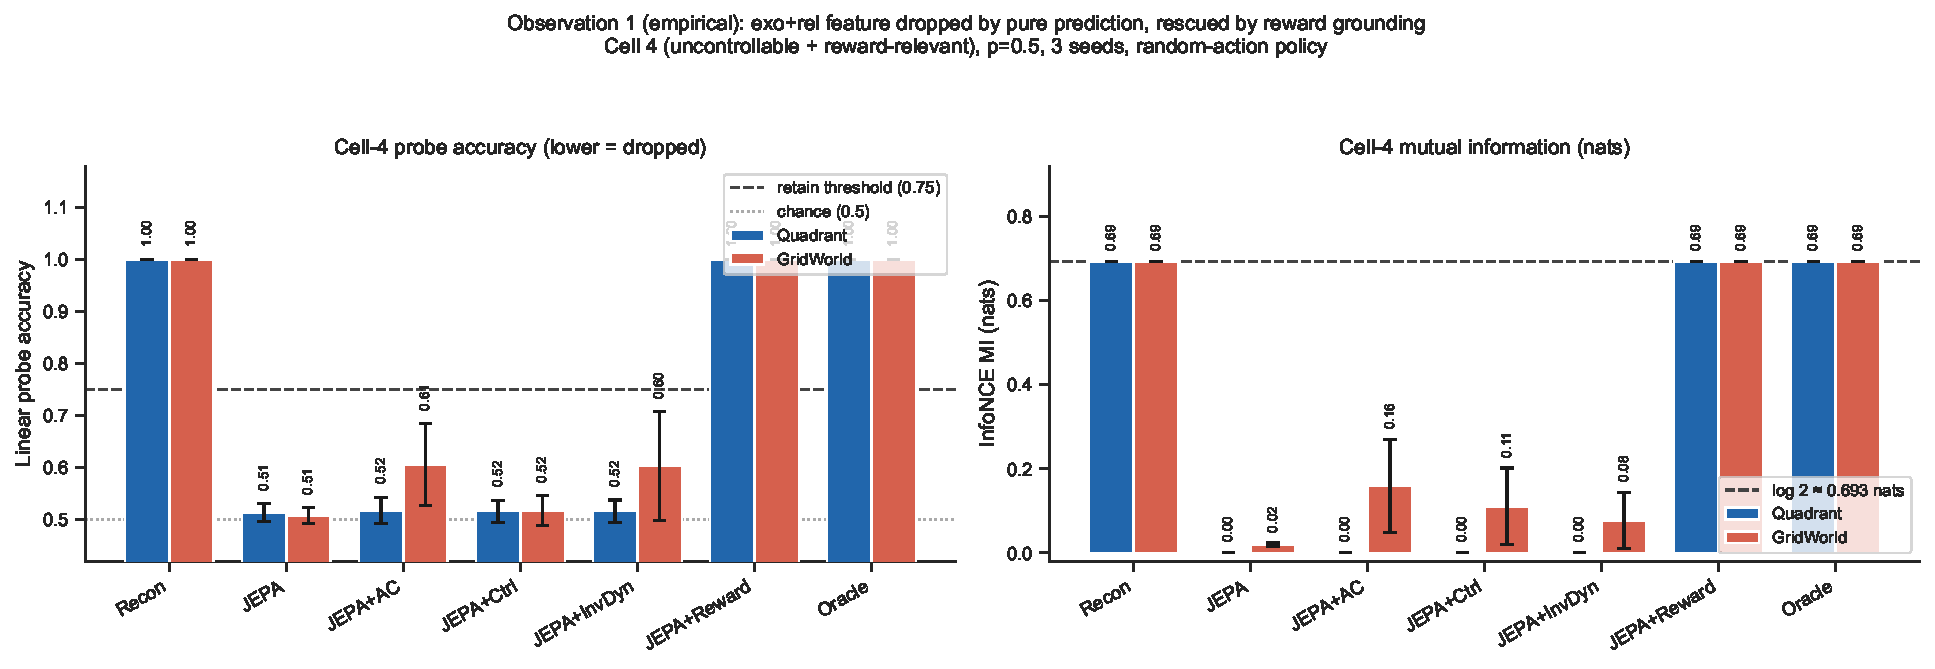
\includegraphics[width=0.95\linewidth]{figure9_cell4_failure_both_envs.pdf}
\caption{\textbf{Cell-4 failure across both environments.} Left: \probe{} (chance $=0.50$, retain
threshold $=0.75$) for each objective on the exogenous control-relevant feature. Right: InfoNCE
mutual information (nats; $\log 2\approx0.693$ is the maximum for a one-bit feature). Every
reward-free self-prediction objective---including action-conditioned JEPA, controllability-based
JEPA, and inverse dynamics with random actions---fails to retain the feature (probe at chance,
MI $\approx 0$). Reward-grounded prediction recovers it at the theoretical ceiling, matching the
\texttt{recon} and \texttt{oracle} upper bounds. Bars are mean $\pm$ std over three seeds.}
\label{fig:cell4}
\end{figure}

Every self-prediction objective that does not consume a reward signal fails to retain the exogenous
control-relevant feature, in both environments, across three seeds. The complete picture is in
Figure~\ref{fig:cell4} and Table~\ref{tab:cell4_failure}. On \texttt{QuadrantEnv}, \texttt{jepa}
reaches \probe{} $0.51\pm0.02$ with mutual information $0.00\pm0.00$ nats; \texttt{jepa\_ac}
$0.52\pm0.03$; \texttt{jepa\_ctrl} $0.52\pm0.02$; and \texttt{jepa\_invdyn} (random policy)
$0.52\pm0.02$, all at chance with essentially zero retained information
(Table~\ref{tab:cell4_failure}). In contrast, \texttt{jepa\_reward} reaches $1.00\pm0.00$ with
$0.69\pm0.00$ nats---the one-bit ceiling---matching the \texttt{recon} and \texttt{oracle} upper
bounds.

\begin{table}[t]
\centering
\caption{Cell-4 failure across both environments (mean\,$\pm$\,std, 3 seeds, random-action policy). Probe acc\,$<$\,0.75 = feature dropped. MI in nats; log\,2\,$\approx$\,0.693 = fully retained. Note large std for \texttt{jepa\_invdyn}: its rescue tracks action informativeness rather than the feature itself.}
\label{tab:cell4_failure}
\begin{tabular}{lcccc}
\toprule
 & \multicolumn{2}{c}{\textbf{Quadrant}} & \multicolumn{2}{c}{\textbf{GridWorld}} \\
\cmidrule(lr){2-3}\cmidrule(lr){4-5}
\textbf{Objective} & Probe acc & MI (nats) & Probe acc & MI (nats) \\
\midrule
  \texttt{recon} & $1.00 \pm 0.00$ & $0.69 \pm 0.00$ & $1.00 \pm 0.00$ & $0.69 \pm 0.00$ \\
  \texttt{jepa} & $0.51 \pm 0.02$ & $0.00 \pm 0.00$ & $0.51 \pm 0.02$ & $0.02 \pm 0.00$ \\
  \texttt{jepa\_ac} & $0.52 \pm 0.03$ & $0.00 \pm 0.00$ & $0.61 \pm 0.08$ & $0.16 \pm 0.11$ \\
  \texttt{jepa\_ctrl} & $0.52 \pm 0.02$ & $0.00 \pm 0.00$ & $0.52 \pm 0.03$ & $0.11 \pm 0.09$ \\
  \texttt{jepa\_invdyn} & $0.52 \pm 0.02$ & $0.00 \pm 0.00$ & $0.60 \pm 0.10$ & $0.08 \pm 0.07$ \\
  \texttt{jepa\_reward} & $1.00 \pm 0.00$ & $0.69 \pm 0.00$ & $1.00 \pm 0.00$ & $0.69 \pm 0.00$ \\
  \texttt{oracle} & $1.00 \pm 0.00$ & $0.69 \pm 0.00$ & $1.00 \pm 0.00$ & $0.69 \pm 0.00$ \\
\bottomrule
\end{tabular}
\end{table}

The picture is the same on \texttt{GridWorldHiddenRuleEnv}, with two informative wrinkles. First,
the order is preserved: \texttt{jepa} sits at $0.51\pm0.02$ and \texttt{jepa\_reward} at
$1.00\pm0.00$. Second, the action-using objectives are noticeably noisier on this richer surface
form---\texttt{jepa\_ac} reaches $0.61\pm0.08$ and \texttt{jepa\_invdyn} $0.60\pm0.10$
(Table~\ref{tab:cell4_failure}). The large standard deviations are themselves the point: on some
seeds the random actions happened to carry marginal information about the rule bit, which is
exactly what the \texttt{jepa\_invdyn} caveat predicts---its retention tracks action
informativeness rather than the feature itself. We therefore report these as mean $\pm$ std and
never as a mean alone.

\paragraph{The feature is dropped, not collapsed.} On \texttt{QuadrantEnv} every dropping objective
retains a high effective rank, between $38$ and $42$; the representation is rich, it has simply
discarded this one feature. On \texttt{GridWorldHiddenRuleEnv} the dropping objectives have
effective rank near $3$ (range $2.75$--$4.61$ across all cell-4 runs), but this reflects the
intrinsic dimensionality of the simpler images rather than collapse: \texttt{recon} retains the
feature perfectly at effective rank $3.30$. ``Low-rank environment'' and ``collapsed
representation'' are distinct, and only the latter would undercut the claim; here the environment is
simply low-dimensional while the feature-dropping is selective.

\begin{figure}[t]
\centering
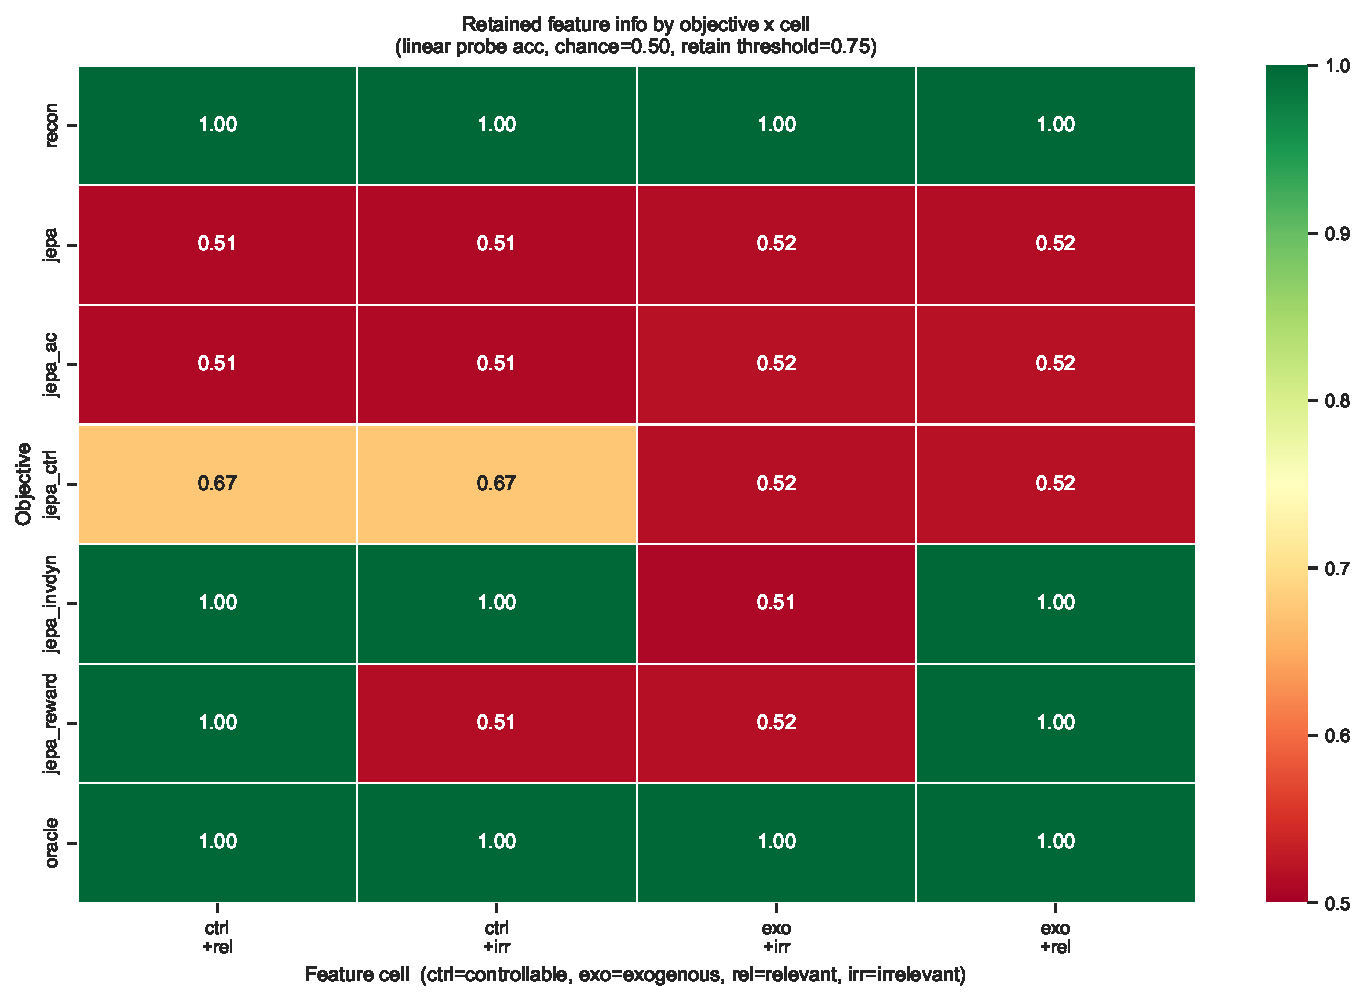
\includegraphics[width=0.64\linewidth]{figure6_quadrant_matrix.pdf}
\caption{\textbf{Full quadrant matrix} of \probe{} per objective $\times$ cell on
\texttt{QuadrantEnv}. Green denotes retained ($\geq0.75$), red denotes dropped ($<0.75$).
\texttt{jepa\_reward} retains exactly the relevant cells (1 and 4) and drops the irrelevant ones (2
and 3); \texttt{jepa\_ctrl} partially recovers the controllable cells (1--2, $\approx0.67$) and
drops the exogenous ones; all purely self-predictive objectives drop every feature under
random-policy data. Cell~4 is the column where only reward grounding survives.}
\label{fig:matrix}
\end{figure}

The full objective $\times$ cell matrix (Figure~\ref{fig:matrix}, with numerical values in
Table~\ref{tab:quadrant_matrix}, Appendix~\ref{app:full}) places cell~4 in context: across the
seven rows, the only objectives that retain the exogenous control-relevant feature are
\texttt{jepa\_reward} and the two upper bounds (\texttt{recon}, \texttt{oracle}).

\subsection{Reward grounding is selectively relevant, not selectively controllable}
\label{sec:selective}

The fix does not merely retain cell~4; it retains the right \emph{axis}. \texttt{jepa\_reward}
keeps both relevant cells---cell~1 (controllable) and cell~4 (exogenous)---and drops both
irrelevant cells---cell~2 and cell~3 (Figure~\ref{fig:matrix}, Table~\ref{tab:quadrant_matrix}).
Its mutual information is $0.693$ nats exactly where the probe is $1.00$ and $0$ nats exactly where
the probe is $\approx0.51$, with zero variance across seeds. Its selectivity axis is relevance.

Contrast this with the controllability-based objective. \texttt{jepa\_ctrl} keeps cells~1 and~2
(both \emph{controllable}, relevant or not, at $\approx0.67$) and drops cells~3 and~4 (both
exogenous). Its selectivity axis is controllability---the wrong axis for control performance,
because it spends capacity on a controllable-irrelevant feature while discarding the
exogenous-relevant one. The distinction between controllability-based and reward-based selectivity
is not semantic: \texttt{jepa\_ctrl} fails to retain the exogenous control-relevant feature while
wasting capacity on the controllable-irrelevant one. (We note that the \texttt{jepa\_ctrl} cell-1/2
value of $0.67\pm0.23$ is driven by a single seed reaching $1.00$ while the others stay near chance,
so it is a partial and unstable recovery, not a clean retain; Table~\ref{tab:quadrant_matrix}.)

\subsection{The failure is not a capacity problem}
\label{sec:capacity}

\begin{figure}[t]
\centering
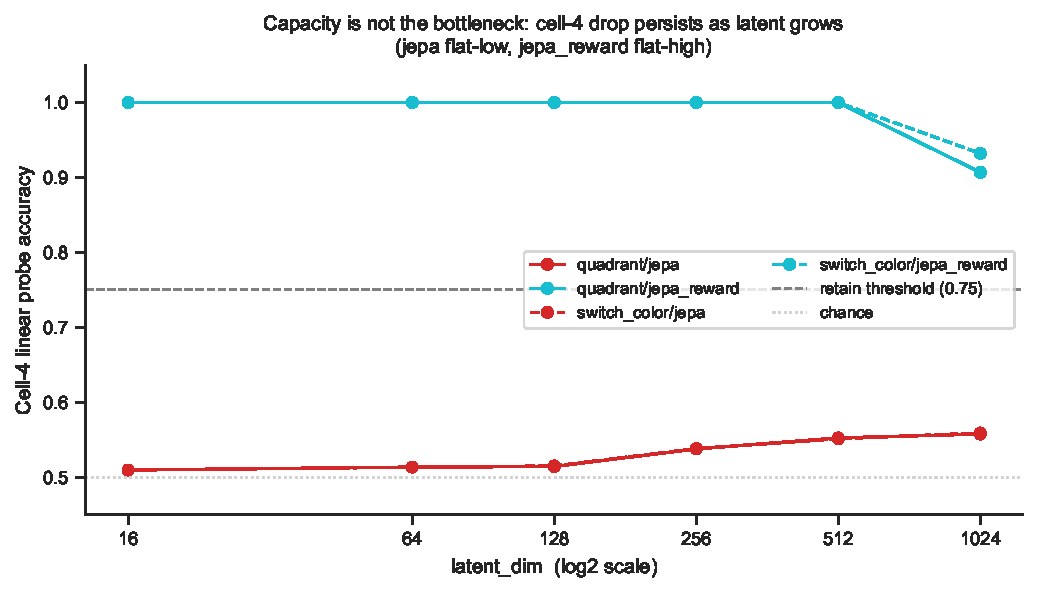
\includegraphics[width=0.7\linewidth]{figure8_capacity.pdf}
\caption{\textbf{Cell-4 retention versus latent dimension} for \texttt{jepa} and
\texttt{jepa\_reward} on \texttt{QuadrantEnv} and \texttt{SwitchColor}. JEPA stays near chance
across every latent dimension from $16$ to $1024$, never approaching the retain threshold.
\texttt{jepa\_reward} stays near perfect from $16$ to $512$, with a slight dip at $1024$
attributable to training budget at that scale. The failure is objective-structural, not
architectural.}
\label{fig:capacity}
\end{figure}

Increasing latent capacity does not rescue the feature for JEPA. As the latent
dimension grows from $16$ to $1024$, JEPA's cell-4 \probe{} moves only from $0.510$ to $0.558$ on
\texttt{QuadrantEnv}---never crossing the $0.75$ retain threshold (Figure~\ref{fig:capacity},
Table~\ref{tab:capacity_minreward}). The slight upward drift at very large dimensions is small and
plausibly reflects marginal saturation of the covariance regularizer rather than genuine retention.
\texttt{jepa\_reward} holds at $1.00$ from dimension $16$ through $512$ and dips to $0.907$
(\texttt{Quadrant}) / $0.932$ (\texttt{SwitchColor}) only at $1024$, a training-budget artifact at
the largest scale rather than a capacity floor. The cell-4 drop is a property of the objective, not
of the encoder's size.

\subsection{Reward grounding is label-efficient}
\label{sec:labeleff}

\begin{figure}[t]
\centering
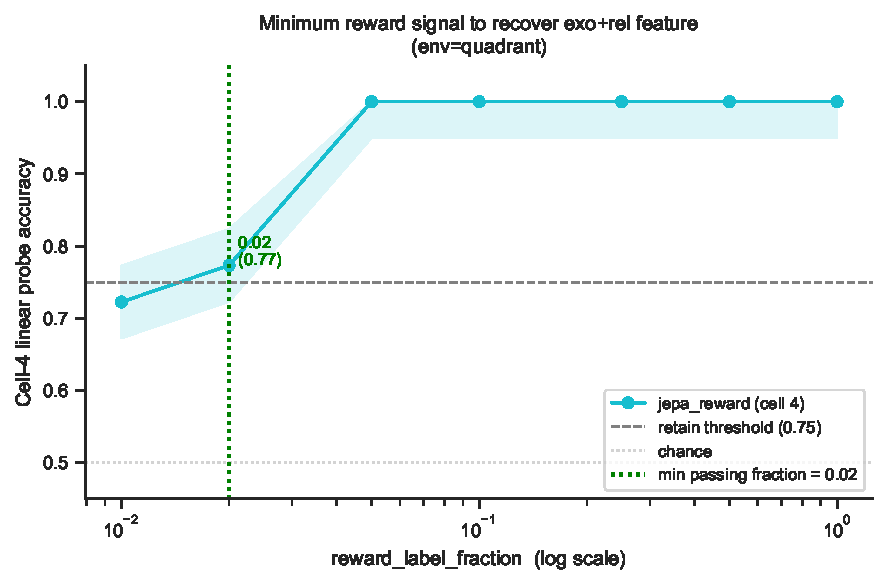
\includegraphics[width=0.7\linewidth]{figure7_min_reward_signal_quadrant.pdf}
\caption{\textbf{Cell-4 retention versus the fraction of reward-labeled transitions} (log scale,
\texttt{QuadrantEnv}). The retain threshold ($0.75$) is first crossed at a reward-label fraction of
$0.02$---two percent of transitions (mean accuracy $0.77$). Even $1\%$ of labeled transitions
yields \probe{} $0.72$, already well above the chance level of $0.50$. The reward signal is highly
efficient for recovering the exogenous control-relevant feature.}
\label{fig:minreward}
\end{figure}

The reward signal is also cheap. The smallest reward-label fraction for which \texttt{jepa\_reward}
crosses the retain threshold is $0.02$---one labeled transition in fifty, at mean accuracy $0.77$
(Figure~\ref{fig:minreward}, Table~\ref{tab:capacity_minreward}). At a fraction of $0.01$ (one in a
hundred) the probe is already $0.72$, substantially above the chance level of $0.50$. This
efficiency suggests that the sparse reward signals available in many real environments may be
sufficient to prevent the failure even when dense reward annotation is not available.

% ===========================================================================
\section{Observation 1 (Empirical)}
\label{sec:obs1}
% ===========================================================================

\begin{quote}
\textbf{Observation 1 (empirical).} At convergence of the JEPA self-prediction objective on the
exogenous control-relevant cell (cell~4, $p_{\text{repeat}}=0.5$), the class-conditional centroid
distance between $c=0$ and $c=1$ state representations in the learned latent space is $0.105$, while
the analytically-derived on-policy bisimulation distance between the same classes is $1.0$. The
\emph{bisimulation error}---the gap between the analytical distance and the realized latent
distance---is $1.893$ out of a maximum of $\approx2.0$. The oracle and reconstruction baselines
realize $1.998$ of the maximum class separation; JEPA realizes about $5\%$ of the oracle's.
\end{quote}

\begin{figure}[t]
\centering
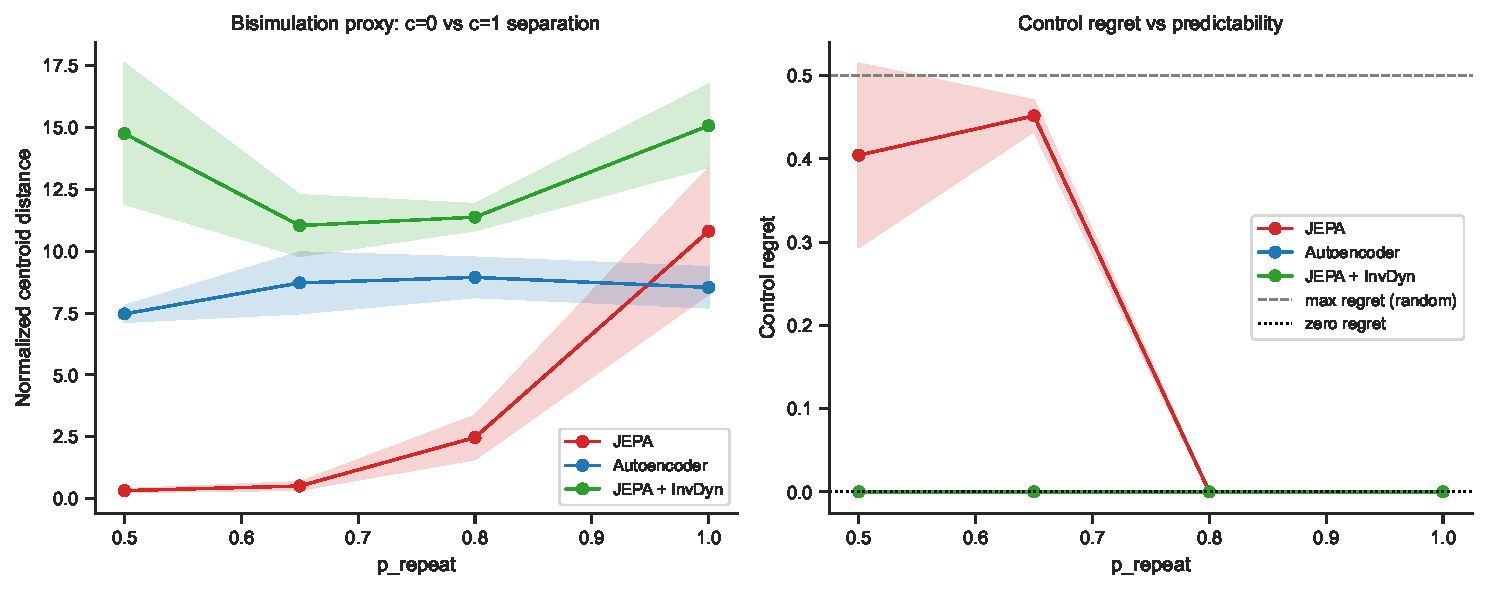
\includegraphics[width=0.58\linewidth]{figure2_bisimulation.pdf}
\caption{\textbf{Class separation} (centroid distance between $c=0$ and $c=1$ latent
representations) for \texttt{jepa}, \texttt{recon}, and \texttt{oracle} at convergence (cell~4,
$p_{\text{repeat}}=0.5$, full training). The horizontal reference marks the analytical bisimulation
distance ($1.0$). JEPA realizes only about $5\%$ of the oracle's class separation ($0.105$ versus
$1.998$); the resulting bisimulation error is $1.893$.}
\label{fig:bisim}
\end{figure}

The cell-4 feature has analytical on-policy bisimulation distance $1.0>0$: the immediate-reward gap
is $1.0$ and the discounted exogenous-transition term vanishes at $p_{\text{repeat}}=0.5$, so
bisimulation theory says the feature must be kept. Only the reward-grounded oracle and the
pixel-grounded reconstruction baseline realize that separation in latent space (class distance
$\approx1.998$); the JEPA latent realizes only $0.105$, about $5\%$ of the oracle's, and its
\probe{} sits at chance ($0.49$). The bisimulation error---oracle minus JEPA, $1.893$---stays
near-maximal at convergence (Figure~\ref{fig:bisim}). Latent self-prediction has no gradient toward
an unpredictable-but-relevant feature and collapses it even though it is trivially encodable. These
proposition numbers are a single-seed point estimate under full training and are reported as such.

\begin{figure}[t]
\centering
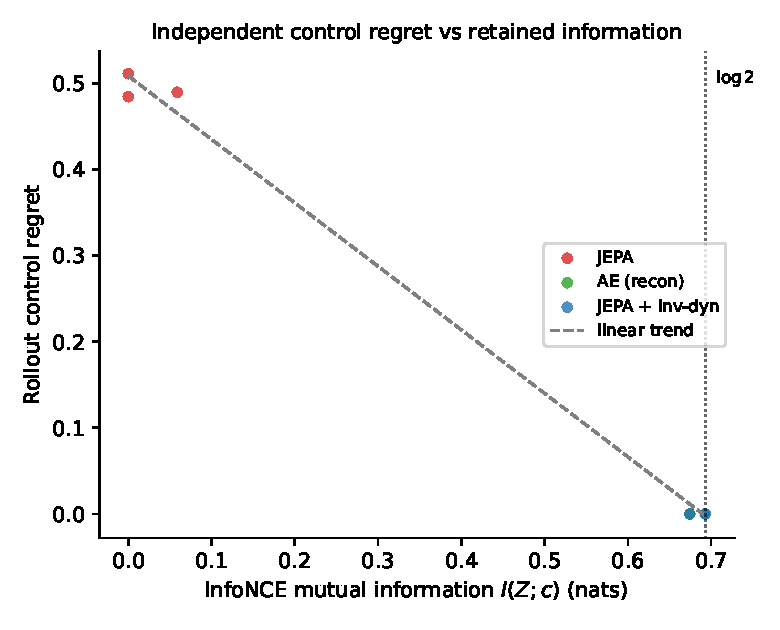
\includegraphics[width=0.66\linewidth]{figure3b_regret_vs_mi.pdf}
\caption{\textbf{Independent control regret versus retained information.} For each run of the
\texttt{SwitchColor} predictability sweep (\texttt{jepa}, \texttt{ae}, \texttt{jepa\_invdyn};
$p_{\text{repeat}}\in\{0.5,0.65,0.8,1.0\}$; two seeds), the horizontal axis is the InfoNCE mutual
information $I(Z;c)$ estimated by a separate critic, and the vertical axis is the regret of an
\emph{independent} behaviour-cloned policy rolled out in the environment. Neither quantity is
derived from the linear probe, so the relationship is non-circular. Runs that retain the feature
($\mathrm{MI}$ saturating at $\log 2$) incur zero control regret; runs that drop it
($\mathrm{MI}\approx 0$) incur chance-level regret ($\approx 0.49$); the off-diagonal is empty
(Pearson $r=-0.999$). This is a separate, reduced-budget run (2000 training steps), reported
distinctly from the full-training numbers elsewhere in the paper (Section~\ref{sec:limits}).}
\label{fig:theory}
\end{figure}

\citet{zhang2020dbc} relate bisimulation-aligned representations to lower control regret, and
Figure~\ref{fig:theory} confirms that link with two measurements that are both independent of the
linear probe: an InfoNCE estimate of $I(Z;c)$, and the regret of a separate behaviour-cloned policy
rolled out in the environment. Across the predictability sweep the two are almost perfectly
anti-correlated (Pearson $r=-0.999$): every run that retains the feature
($\mathrm{MI}\approx\log 2$) achieves zero control regret, while every run that drops it
($\mathrm{MI}\approx 0$) is stuck at chance-level control ($\approx 0.49$), with no run in between.
Because neither axis is derived from the probe, this is independent evidence---not the definitional
$\text{regret}=1-\text{accuracy}$ identity---that the information a reward-free self-prediction
objective discards is exactly the information a controller needs. The relationship is a sharp
threshold rather than a smooth dose--response, as expected for a one-bit feature. Together with
Observation~1---the near-zero class separation and near-maximal bisimulation error measured directly
from the latent geometry---this shows the failure is structural rather than incidental.

We emphasize that Observation~1 is an empirical measurement in a controlled synthetic environment,
not a formal proof; the analytical bisimulation distance is a closed-form derivation, but the claim
that JEPA collapses the feature is measured from trained models on a finite budget, and its
generality to large pretrained JEPA models is an open question.

% ===========================================================================
\section{Related Work and Discussion}
% ===========================================================================

\subsection{JEPA and world models}
I-JEPA~\citep{assran2023ijepa}, V-JEPA 2 and V-JEPA 2-AC~\citep{vjepa2_2025}, and
DINO-WM~\citep{zhou2024dinowm} establish the latent-prediction objective and demonstrate its
empirical benefits for representation learning and planning on pre-trained visual features. These
works motivate the objective; our work is complementary, asking what information is structurally at
risk under it.

\subsection{Bisimulation-based representation learning}
DBC~\citep{zhang2020dbc} established that bisimulation-aligned representations are far more robust to
task-irrelevant distractors than reconstruction, by explicitly factoring out reward-irrelevant
variation. DeepMDP~\citep{gelada2019deepmdp} learns latent models with reward and transition losses
that provably bound value error, and action-bisimulation~\citep{actionbisim2024} extends
bisimulation to action-conditioned settings. These lines established that the reward signal shapes
which structure a representation keeps; our contribution is the controlled isolation of the specific
cell where self-prediction and bisimulation conflict---exogenous and relevant---and a quantitative
measurement of the information gap.

\subsection{Closest prior work}
\paragraph{Bisimulation on JEPA world models (arXiv:2602.18639).}
\citet{bisimjepa2026} apply a bisimulation objective to JEPA world models to handle distractors. We
differ in the cell we target: their distractors are exogenous
and \emph{irrelevant} (cell~3), the classic distractor the agent neither controls nor needs, whereas
we target the exogenous and \emph{relevant} cell~4. Their bisimulation grounding and our reward
grounding are related fixes, but they are motivated by different failure modes.

\paragraph{Sensorimotor world models (arXiv:2606.20104).}
\citet{sensorimotor2026} add an inverse-dynamics regularizer to retain action-relevant features.
Our \texttt{jepa\_invdyn} (random-policy) experiment shows directly that
when actions do not encode the exogenous-relevant feature, inverse dynamics fails: cell-4 retention
is only $0.52\pm0.02$ on \texttt{QuadrantEnv} (Table~\ref{tab:cell4_failure}). That fix works for
controllable features but does not generalize to exogenous-relevant ones without an informative
policy.

\paragraph{A critique of world models (arXiv:2507.05169).}
\citet{xing2025critique} name task-relevant information loss as a concern for JEPA-style models. We
make that concern concrete by measuring it---mutual information, bisimulation error, and probe
accuracy---in controlled isolation, and by exhibiting a selective fix.

\subsection{Limitations}
\label{sec:limits}
\begin{itemize}
  \item All results are in controlled synthetic environments with $12\times12$ (and $32\times32$)
  observations. Real-model transfer to large pretrained JEPA encoders (e.g.\ V-JEPA 2-AC) has not
  been tested and is future work.
  \item Observation~1 is empirical, not a proved theorem; a theorem would require explicit
  assumptions about the learning dynamics and the environment class.
  \item The gridworld environment has intrinsically low-rank observations (effective rank
  $\approx3$); the effective-rank anti-collapse check is calibrated for the quadrant environment
  and should be interpreted differently there.
  \item The \texttt{jepa\_invdyn} result depends on the action policy: the cell-4 failure holds
  under random actions but need not hold under every informative policy.
  \item The regret-versus-information result (Figure~\ref{fig:theory}) is de-circularized---both
  axes are independent of the linear probe---but was produced by a separate, reduced-budget run
  ($2000$ training steps on CPU, two seeds), not the full-training regime used elsewhere; and
  because the feature is one bit, the relationship is a sharp threshold, so the near-perfect Pearson
  correlation should be read as ``retain $\Rightarrow$ zero regret, drop $\Rightarrow$ chance-level
  regret,'' not as a smooth dose--response.
\end{itemize}

\subsection{Future work}
The natural next step is to demonstrate the failure mode on a pretrained V-JEPA 2-AC or DINO-WM
encoder in a goal-not-given task. The minimal-reward-signal result ($2\%$ of transitions) suggests
that even a weakly reward-conditioned adapter on a frozen JEPA encoder may be enough to prevent it.

% ===========================================================================
\appendix
\section{Environment implementation details}
\label{app:env}
\texttt{QuadrantEnv} renders $12\times12$ grayscale frames: a $3\times3$ corner patch carries the
feature bit, and the background is a sum of four spatial-frequency gratings whose phase advances
deterministically each step, giving the encoder predictable structure to model. \texttt{FeatureSpec}
records, per feature, whether it is controllable (toggled by the action) and whether it is relevant
(sets the reward), and \texttt{make\_cell(cell, predictability)} assembles the single-feature spec
for each quadrant cell. Exogenous features evolve with $P(c_{t+1}=c_t)=p_{\text{repeat}}$; the
optimal action is $a^\ast=c_t$ and the reward is $1$ iff the action matches the relevant bit. The
main experiments use $20000$ training transitions, $4000$ evaluation transitions, batch size $128$,
learning rate $10^{-3}$, latent dimension $128$, $4000$ training steps, and seeds $\{0,1,2\}$. The
two replication surface forms are \texttt{SwitchColorEnv} ($32\times32$, intensity patch over a
sinusoidal grating) and \texttt{GridWorldHiddenRuleEnv} (bottom-right patch over a drifting texture
with an agent marker). As a check on the predictability knob in \texttt{SwitchColorEnv}, JEPA
recovers the feature at $1.00\pm0.00$ when $p_{\text{repeat}}=1.0$ and only $0.61\pm0.13$ when
$p_{\text{repeat}}=0.5$, while reconstruction holds at $1.00\pm0.00$ throughout.

\section{InfoNCE estimator details}
\label{app:infonce}
The mutual-information estimate is a separable InfoNCE critic (a small MLP) trained on a held-out
split so the bound stays honest~\citep{oord2018cpc}, run for $300$ epochs. As a sanity check, the
estimator returns approximately $\log 2\approx0.69$ nats when the feature is perfectly recoverable
and approximately $0$ nats when the feature is independent of the latent, matching the values
observed for \texttt{recon}/\texttt{oracle} and for collapsed JEPA latents respectively
(Table~\ref{tab:cell4_failure}).

\section{Full results}
\label{app:full}
Table~\ref{tab:quadrant_matrix} gives the full objective $\times$ cell matrix on
\texttt{QuadrantEnv} (mean $\pm$ std over three seeds). In this matrix \texttt{jepa\_invdyn} is
trained on informative-action data ($a^\ast$ with $\varepsilon=0.2$ exploration); its cell-4
retention of $1.00$ there tracks action informativeness, not reward grounding, and under random
actions it drops to chance (Table~\ref{tab:cell4_failure}). Table~\ref{tab:capacity_minreward} gives
the capacity sweep across both environments and the minimum reward-label fraction.

\begin{table}[t]
\centering
\caption{Full objective $\times$ cell retention matrix. Values are linear probe accuracy (mean\,$\pm$\,std over 3 seeds, chance\,=\,0.50). Highlighted: cell 4 (exo\,+\,rel), the hard case where only reward-grounded signals retain the feature.}
\label{tab:quadrant_matrix}
\begin{tabular}{lcccc}
\toprule
\textbf{Objective} & \makecell{\textbf{Cell 1}\\\\\textbf{ctrl+rel}} & \makecell{\textbf{Cell 2}\\\\\textbf{ctrl+irr}} & \makecell{\textbf{Cell 3}\\\\\textbf{exo+irr}} & \makecell{\textbf{Cell 4}\\\\\textbf{exo+rel}} \\
\midrule
  \texttt{recon} & $1.00 \pm 0.00$ & $1.00 \pm 0.00$ & $1.00 \pm 0.00$ & $1.00 \pm 0.00$ \\
  \texttt{jepa} & $0.51 \pm 0.01$ & $0.51 \pm 0.01$ & $0.52 \pm 0.02$ & $0.52 \pm 0.02$ \\
  \texttt{jepa\_ac} & $0.51 \pm 0.01$ & $0.51 \pm 0.01$ & $0.52 \pm 0.03$ & $0.52 \pm 0.03$ \\
  \texttt{jepa\_ctrl} & $0.67 \pm 0.23$ & $0.67 \pm 0.23$ & $0.52 \pm 0.02$ & $0.52 \pm 0.02$ \\
  \texttt{jepa\_invdyn} & $1.00 \pm 0.00$ & $1.00 \pm 0.00$ & $0.51 \pm 0.03$ & $1.00 \pm 0.00$ \\
  \texttt{jepa\_reward} & $1.00 \pm 0.00$ & $0.51 \pm 0.01$ & $0.52 \pm 0.02$ & $1.00 \pm 0.00$ \\
  \texttt{oracle} & $1.00 \pm 0.00$ & $1.00 \pm 0.00$ & $1.00 \pm 0.00$ & $1.00 \pm 0.00$ \\
\bottomrule
\end{tabular}
\end{table}

\begin{table}[t]
\centering
\caption{(Top) Capacity sweep: cell-4 linear probe accuracy vs latent dimension for \texttt{jepa} and \texttt{jepa\_reward} on both environments (3 seeds; values are means where per-seed data is available, else mean only). \texttt{jepa} stays near chance and \texttt{jepa\_reward} stays near perfect across all sizes, ruling out capacity as the bottleneck. (Bottom) Minimum reward-signal fraction: the smallest \texttt{reward\_label\_fraction} for which \texttt{jepa\_reward} retains cell 4 (probe acc\,$\geq$\,0.75) on Quadrant (3 seeds, mean shown).}
\label{tab:capacity_minreward}
\begin{tabular}{lcccc}
\toprule
\textbf{latent\_dim} & \multicolumn{2}{c}{\textbf{Quadrant}} & \multicolumn{2}{c}{\textbf{SwitchColor}} \\
\cmidrule(lr){2-3}\cmidrule(lr){4-5}
 & \texttt{jepa} & \texttt{jepa\_reward} & \texttt{jepa} & \texttt{jepa\_reward} \\
\midrule
  16 & $0.51$ & $1.00$ & $0.51$ & $1.00$ \\
  64 & $0.51$ & $1.00$ & $0.51$ & $1.00$ \\
  128 & $0.51$ & $1.00$ & $0.52$ & $1.00$ \\
  256 & $0.54$ & $1.00$ & $0.54$ & $1.00$ \\
  512 & $0.55$ & $1.00$ & $0.55$ & $1.00$ \\
  1024 & $0.56$ & $0.91$ & $0.56$ & $0.93$ \\
\midrule
\multicolumn{5}{l}{\textit{Minimum reward-label fraction (Quadrant, cell 4)}} \\
\midrule
\textbf{reward\_frac} & \multicolumn{4}{c}{\textbf{Cell-4 probe acc (mean)}} \\
\midrule
  0.01 & $0.72$ &  \\
  0.02 & $0.77$ &  $\leftarrow$ min passing \\
  0.05 & $1.00$ &  \\
  0.1 & $1.00$ &  \\
  0.25 & $1.00$ &  \\
  0.5 & $1.00$ &  \\
  1 & $1.00$ &  \\
\bottomrule
\end{tabular}
\end{table}

\section{Reproducibility}
\label{app:repro}
Results are deterministic given fixed seeds $\{0,1,2\}$ and were produced on a GPU
(CUDA, PyTorch). An automated check (\texttt{verify.py}) asserts the encoder-identity invariant
(matching \texttt{state\_dict} keys and shapes across all objectives) and the evaluation-protocol
invariant (disjoint evaluation seed; probes read the online encoder, never the EMA target), and
exercises the InfoNCE sanity check above. Full reproduction instructions and the per-run result
JSONs that back every full-training number in this paper are described in the accompanying
\texttt{REPRODUCE.md}. The de-circularized regret-versus-information run (Figure~\ref{fig:theory})
is reproduced separately by \texttt{regret\_mi\_experiment.py} (which records \texttt{mi\_infonce}
and \texttt{control\_regret\_rollout} per run to \texttt{regret\_mi\_sweep.json}) and
\texttt{make\_regret\_mi\_figure.py}; it uses a reduced budget of $2000$ training steps on CPU and
seeds $\{0,1\}$.

\bibliographystyle{plainnat}
\bibliography{references}

\end{document}
